\documentclass{article}

%%%%
% PLOTS mapas y conglomerados
% bibliografia
%%%%
\usepackage[utf8]{inputenc}
\usepackage{longtable}
\usepackage{authblk}
\usepackage{adjustbox}

\usepackage{natbib}



\title{LOS INDICES DEL MUNDO}
% autores
\renewcommand\Authand{, y }
\author[1]{\normalsize Maria Luisa Franco}


\affil[1,2]{\small  Escuela de Ingenieria,Universidad de los Andes\\
\texttt{{delcurso,deallado}@uniandes.edu.col}}
\affil[1]{\small Instituto de altas investigaciones financieras\\
Banco del Parque\\
\texttt{delcurso@bp.com.col}}

\date{30 de Junio de 2018}

%%%%
\usepackage{Sweave}
\begin{document}
\Sconcordance{concordance:final.tex:final.Rnw:%
1 30 1 1 0 26 1 1 4 5 0 1 2 3 1 1 3 15 0 1 2 12 1 1 18 1 3 11 1 1 8 12 %
0 1 3 4 1 1 10 1 0 1 4 13 0 1 5 6 1 1 4 1 2 12 1 1 5 1 1 1 4 31 0 1 2 %
11 1 1 9 1 1 1 27 6 1 1 14 2 0 1 14 1 2 17 1}


\maketitle


\begin{abstract}
Este es mi primer trabajo en exploracion y modelamiento de indices usando LATEX. Este trabajo lo he hecho bajo la filosofía de trabajo replicable. Este es mi primer trabajo en exploracion y modelamiento de indices usando LATEX. Este trabajo lo he hecho bajo la filosofía de trabajo replicable. Este es mi primer trabajo en exploracion y modelamiento de indices usando LATEX. Este trabajo lo he hecho bajo la filosofía de trabajo replicable. Este es mi primer trabajo en exploracion y modelamiento de indices usando LATEX. Este trabajo lo he hecho bajo la filosofía de trabajo replicable.
\end{abstract}

\section*{Introducción}

Aqui les presento mi investigacion sobre diversos indices sociales en el mundo. Los indices los conseguí de wikipedia, espero que les gusten mucho. Aqui les presento mi investigacion sobre diversos indices sociales en el mundo. Los indices los conseguí de wikipedia, espero que les gusten mucho.Aqui les presento mi investigacion sobre diversos indices sociales en el mundo. Los indices los conseguí de wikipedia, espero que les gusten mucho.Aqui les presento mi investigacion sobre diversos indices sociales en el mundo. Los indices los conseguí de wikipedia, espero que les gusten mucho.
Aqui les presento mi investigacion sobre diversos indices sociales en el mundo. Los indices los conseguí de wikipedia, espero que les gusten mucho.Aqui les presento mi investigacion sobre diversos indices sociales en el mundo. Los indices los conseguí de wikipedia, espero que les gusten mucho.Aqui les presento mi investigacion sobre diversos indices sociales en el mundo. Los indices los conseguí de wikipedia, espero que les gusten mucho.

Comencemos viendo que hay en la sección \ref{univariada} en la página \pageref{univariada}.

\clearpage



\section{Exploración Univariada}\label{univariada}

En esta sección exploro cada índice. En esta sección exploro cada índice. En esta sección exploro cada índice. En esta sección exploro cada índice. En esta sección exploro cada índice. En esta sección exploro cada índice. En esta sección exploro cada índice. En esta sección exploro cada índice. En esta sección exploro cada índice.



\begin{Schunk}
\begin{Soutput}
[1] "IDH"                 "Departamento"        "Población.Cabecera"
[4] "Población.Resto"    "Población.Total"    "DepartamentoNorm"   
\end{Soutput}
\end{Schunk}


Para conocer el comportamiento de las variables se ha preparado la Tabla \ref{Tfrecuencias}, donde se describe la distribución de las modalidades de cada variable. Los números representan la situación de algun país en ese indicador, donde el mayor valor numérico es la mejor situación.

% Table created by stargazer v.5.2.2 by Marek Hlavac, Harvard University. E-mail: hlavac at fas.harvard.edu
% Date and time: vie, jul 06, 2018 - 10:25:21 a.m.
\begin{table}[!htbp] \centering 
  \caption{Medidas estadisticas} 
  \label{stats} 
\begin{tabular}{@{\extracolsep{5pt}}lccccc} 
\\[-1.8ex]\hline 
\hline \\[-1.8ex] 
Statistic & \multicolumn{1}{c}{N} & \multicolumn{1}{c}{Median} & \multicolumn{1}{c}{Mean} & \multicolumn{1}{c}{Min} & \multicolumn{1}{c}{Max} \\ 
\hline \\[-1.8ex] 
IDH & 32 & 0.804 & 0.802 & 0.691 & 0.879 \\ 
Población.Cabecera & 32 & 717,197 & 1,196,730.000 & 13,090 & 10,070,801 \\ 
Población.Resto & 32 & 268,111.5 & 360,590.300 & 21,926 & 1,428,858 \\ 
Población.Total & 32 & 1,028,429 & 1,557,320.000 & 43,446 & 10,985,285 \\ 
\hline \\[-1.8ex] 
\end{tabular} 
\end{table} 

Como apreciamos en la Tabla \ref{Tfrecuencias}, los países en la mejor situación son los menos, salvo en el caso del \emph{índice de libertas mundial}\footnote{Nótese que esto se puede deber a la {\bf menor} cantidad de categorías.}

\clearpage

Para resaltar lo anterior, tenemos la Figura \ref{barplots} en la página \pageref{barplots}.


%%%%% figure
\begin{figure}[h]
\centering

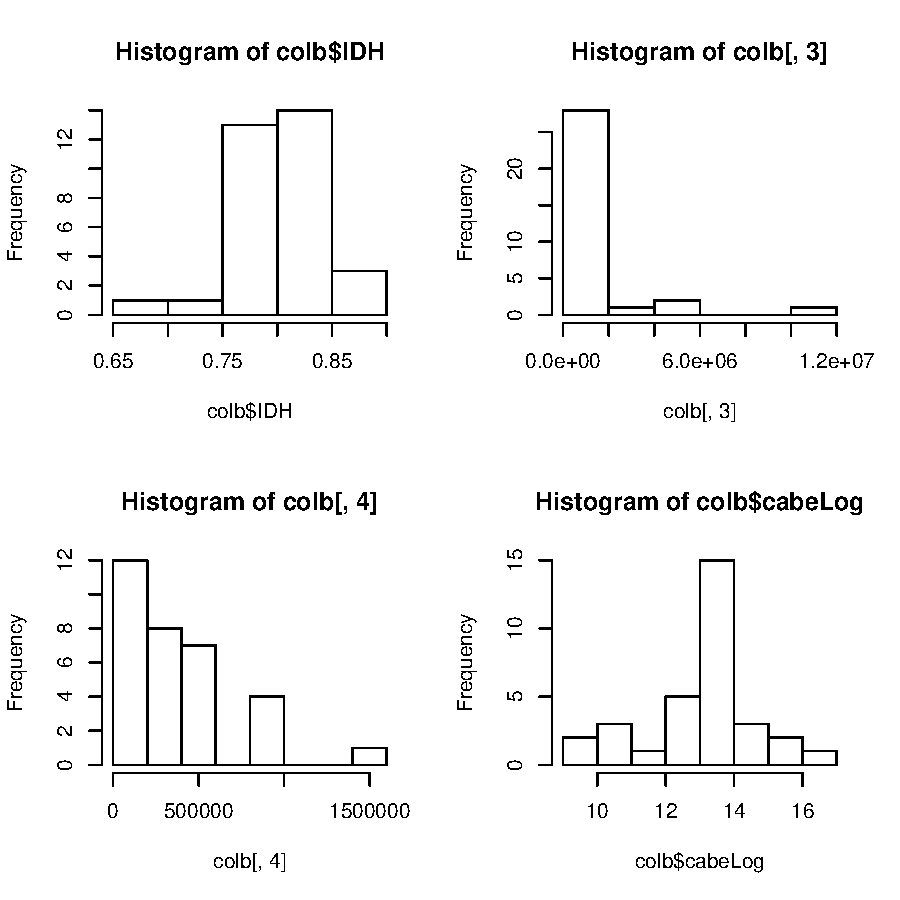
\includegraphics{final-barplots}
 
\caption{Distribución de Indicadores}
\label{barplots}
\end{figure}

Además de la distribución de los variable, es importante saber el valor central. Como los valores son de naturaleza ordinal debemos pedir la {\bf mediana} y otras medidas de posición (como los \emph{cuartiles}, los que no pediremos pues son pocos valores). La mediana de cada variable la mostramos en la Tabla \ref{stats} en la página \pageref{stats}.


\section{Exploración Bivariada}

En este trabajo estamos interesados en el impacto de los otros indices en el nivel de Democracia. Veamos las relaciones bivariadas que tiene esta variable con todas las demás:

% Table created by stargazer v.5.2.2 by Marek Hlavac, Harvard University. E-mail: hlavac at fas.harvard.edu
% Date and time: vie, jul 06, 2018 - 10:25:21 a.m.
\begin{table}[!htbp] \centering 
  \caption{Correlación de IDH con las demás variables} 
  \label{corrDem} 
\begin{tabular}{@{\extracolsep{5pt}} cc} 
\\[-1.8ex]\hline 
\hline \\[-1.8ex] 
cabeLog & restoLog \\ 
\hline \\[-1.8ex] 
$0.487$ & $0.177$ \\ 
\hline \\[-1.8ex] 
\end{tabular} 
\end{table} 

Veamos la correlación entre las variables independientes:


         cabeLog restoLog
cabeLog  "1"     ""      
restoLog "0.84"  "1"     % Table created by stargazer v.5.2.2 by Marek Hlavac, Harvard University. E-mail: hlavac at fas.harvard.edu
% Date and time: vie, jul 06, 2018 - 10:25:21 a.m.
\begin{table}[!htbp] \centering 
  \caption{Correlación entre variables independientes} 
  \label{corrTableX} 
\begin{tabular}{@{\extracolsep{5pt}} ccc} 
\\[-1.8ex]\hline 
\hline \\[-1.8ex] 
 & cabeLog & restoLog \\ 
\hline \\[-1.8ex] 
cabeLog & 1 &  \\ 
restoLog & 0.84 & 1 \\ 
\hline \\[-1.8ex] 
\end{tabular} 
\end{table} 
Lo visto en la Tabla \ref{corrTableX} se refuerza claramente en la Figura \ref{corrPlotX}.

\begin{figure}[h]
\centering
\begin{adjustbox}{width=7cm,height=7cm,clip,trim=1.5cm 0.5cm 0cm 1.5cm}

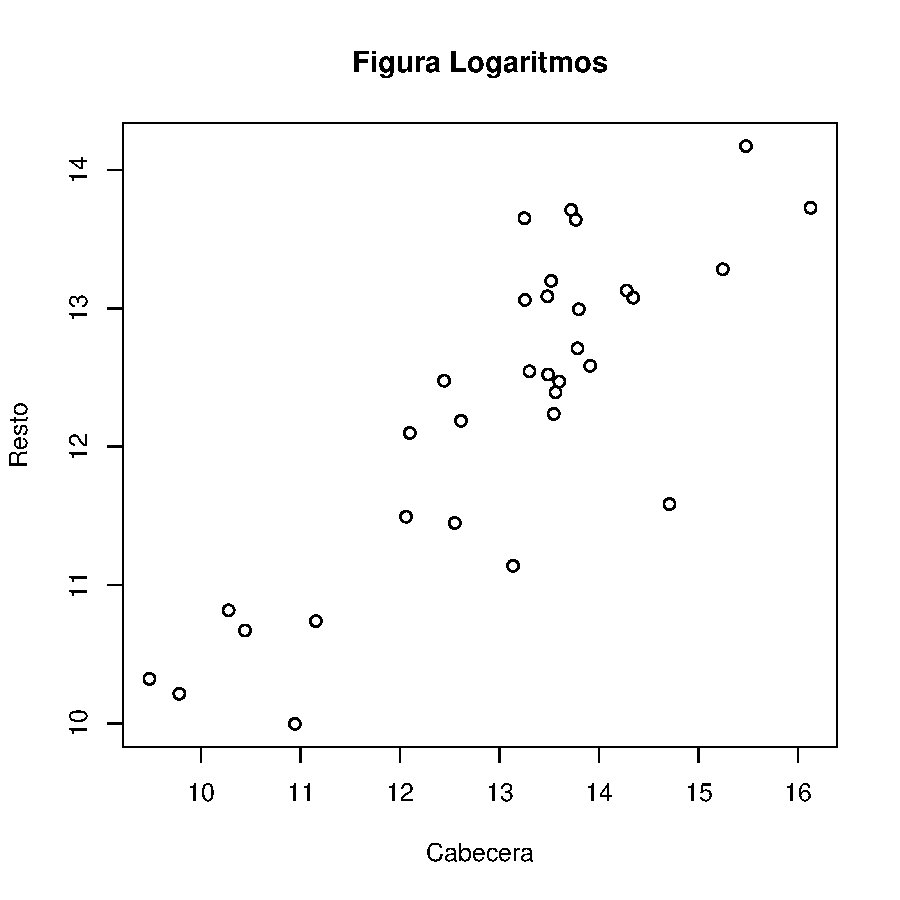
\includegraphics{final-verCorr}

\end{adjustbox}
\caption{correlación entre predictores}
\label{corrPlotX}
\end{figure}


\clearpage

\section{Modelos de Regresión}

Finalmente, vemos los modelos propuestos. Primero sin la libertad mundial como independiente, y luego con está. Los resultados se muestran en la Tabla \ref{regresiones} de la página \pageref{regresiones}.



% Table created by stargazer v.5.2.2 by Marek Hlavac, Harvard University. E-mail: hlavac at fas.harvard.edu
% Date and time: vie, jul 06, 2018 - 10:25:21 a.m.
\begin{table}[!htbp] \centering 
  \caption{Modelos de Regresión} 
  \label{regresiones} 
\begin{tabular}{@{\extracolsep{5pt}}lcc} 
\\[-1.8ex]\hline 
\hline \\[-1.8ex] 
 & \multicolumn{2}{c}{\textit{Dependent variable:}} \\ 
\cline{2-3} 
\\[-1.8ex] & \multicolumn{2}{c}{IDH} \\ 
\\[-1.8ex] & (1) & (2)\\ 
\hline \\[-1.8ex] 
 cabeLog & 0.013$^{***}$ & 0.031$^{***}$ \\ 
  & (0.004) & (0.007) \\ 
  & & \\ 
 restoLog &  & $-$0.030$^{***}$ \\ 
  &  & (0.010) \\ 
  & & \\ 
 Constant & 0.634$^{***}$ & 0.766$^{***}$ \\ 
  & (0.055) & (0.065) \\ 
  & & \\ 
\hline \\[-1.8ex] 
Observations & 32 & 32 \\ 
R$^{2}$ & 0.238 & 0.425 \\ 
Adjusted R$^{2}$ & 0.212 & 0.385 \\ 
Residual Std. Error & 0.037 (df = 30) & 0.033 (df = 29) \\ 
F Statistic & 9.347$^{***}$ (df = 1; 30) & 10.706$^{***}$ (df = 2; 29) \\ 
\hline 
\hline \\[-1.8ex] 
\textit{Note:}  & \multicolumn{2}{r}{$^{*}$p$<$0.1; $^{**}$p$<$0.05; $^{***}$p$<$0.01} \\ 
\end{tabular} 
\end{table} 
Como se vió en la Tabla \ref{regresiones}, cuando está presente el \emph{indice de libertad mundial}, el \emph{índice de libertad de prensa} pierde significancia.

 \clearpage

\section{Exploración Espacial}

Como acabamos de ver en la Tabla \ref{regresiones} en la página \pageref{regresiones}, si quisieras sintetizar la multidimensionalidad de nuestros indicadores, podríamos usar tres de las cuatro variables que tenemos (un par de las originales tiene demasiada correlación).

Así, propongo que calculemos conglomerados de países usando toda la información de tres de los indicadores. Como nuestras variables son ordinales utilizaremos un proceso de conglomeración donde las distancia serán calculadas usando la medida {\bf macqueen} propuestas en \cite{macqueen_methods_nodate}
Los tres conglomerados se muestran en la Figura \ref{clustmap}.






\begin{figure}[h]
\centering
\begin{adjustbox}{width=15cm,height=13cm,clip,trim=25cm 0cm 0cm 0cm}

[1] 2 3 1  Group.1       IDH  cabeLog restoLog
1       1 0.7710833 13.28360 12.89513
2       2 0.7825714 10.58974 10.60684
3       3 0.8406154 14.12024 12.64415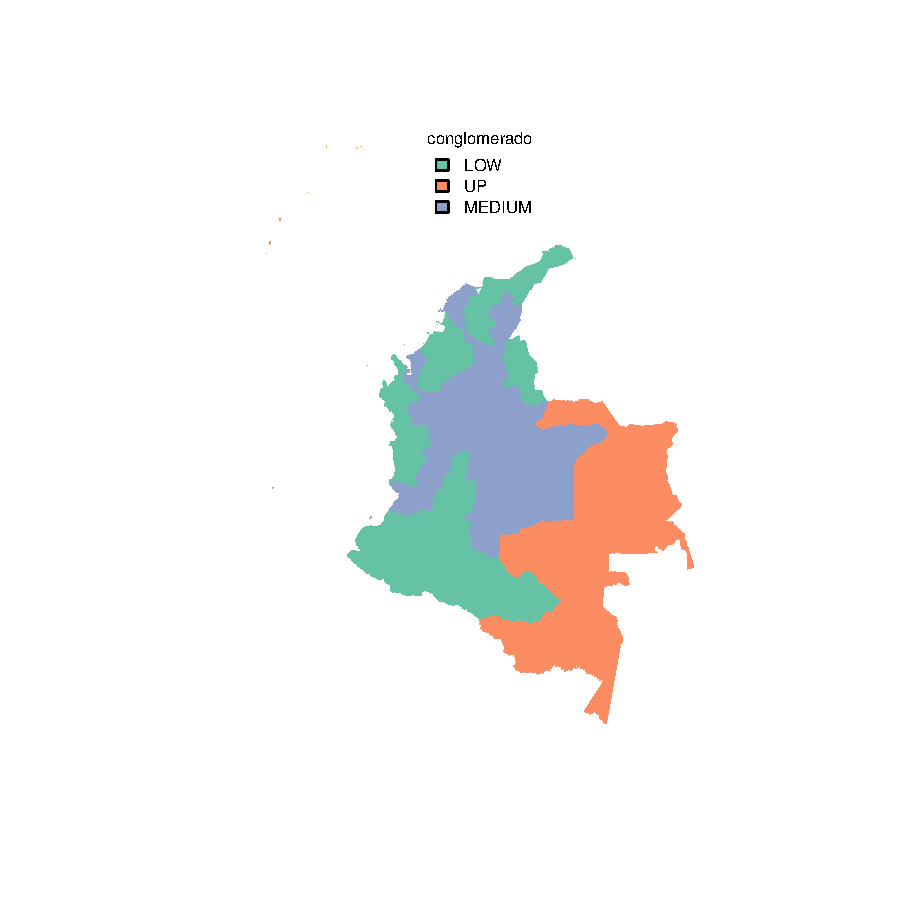
\includegraphics{final-plotMapf}

\end{adjustbox}
\caption{Paises conglomerados segun sus indicadores sociopolaticos}\label{clustmap}
\end{figure}


\bibliographystyle{abbrv}
\renewcommand{\refname}{Bibliografia}
\bibliography{Colombia}

\end{document}
